\section{{\tool}: Model Architecture}
\label{sec:overview}

\begin{figure*}[t]
\begin{center}
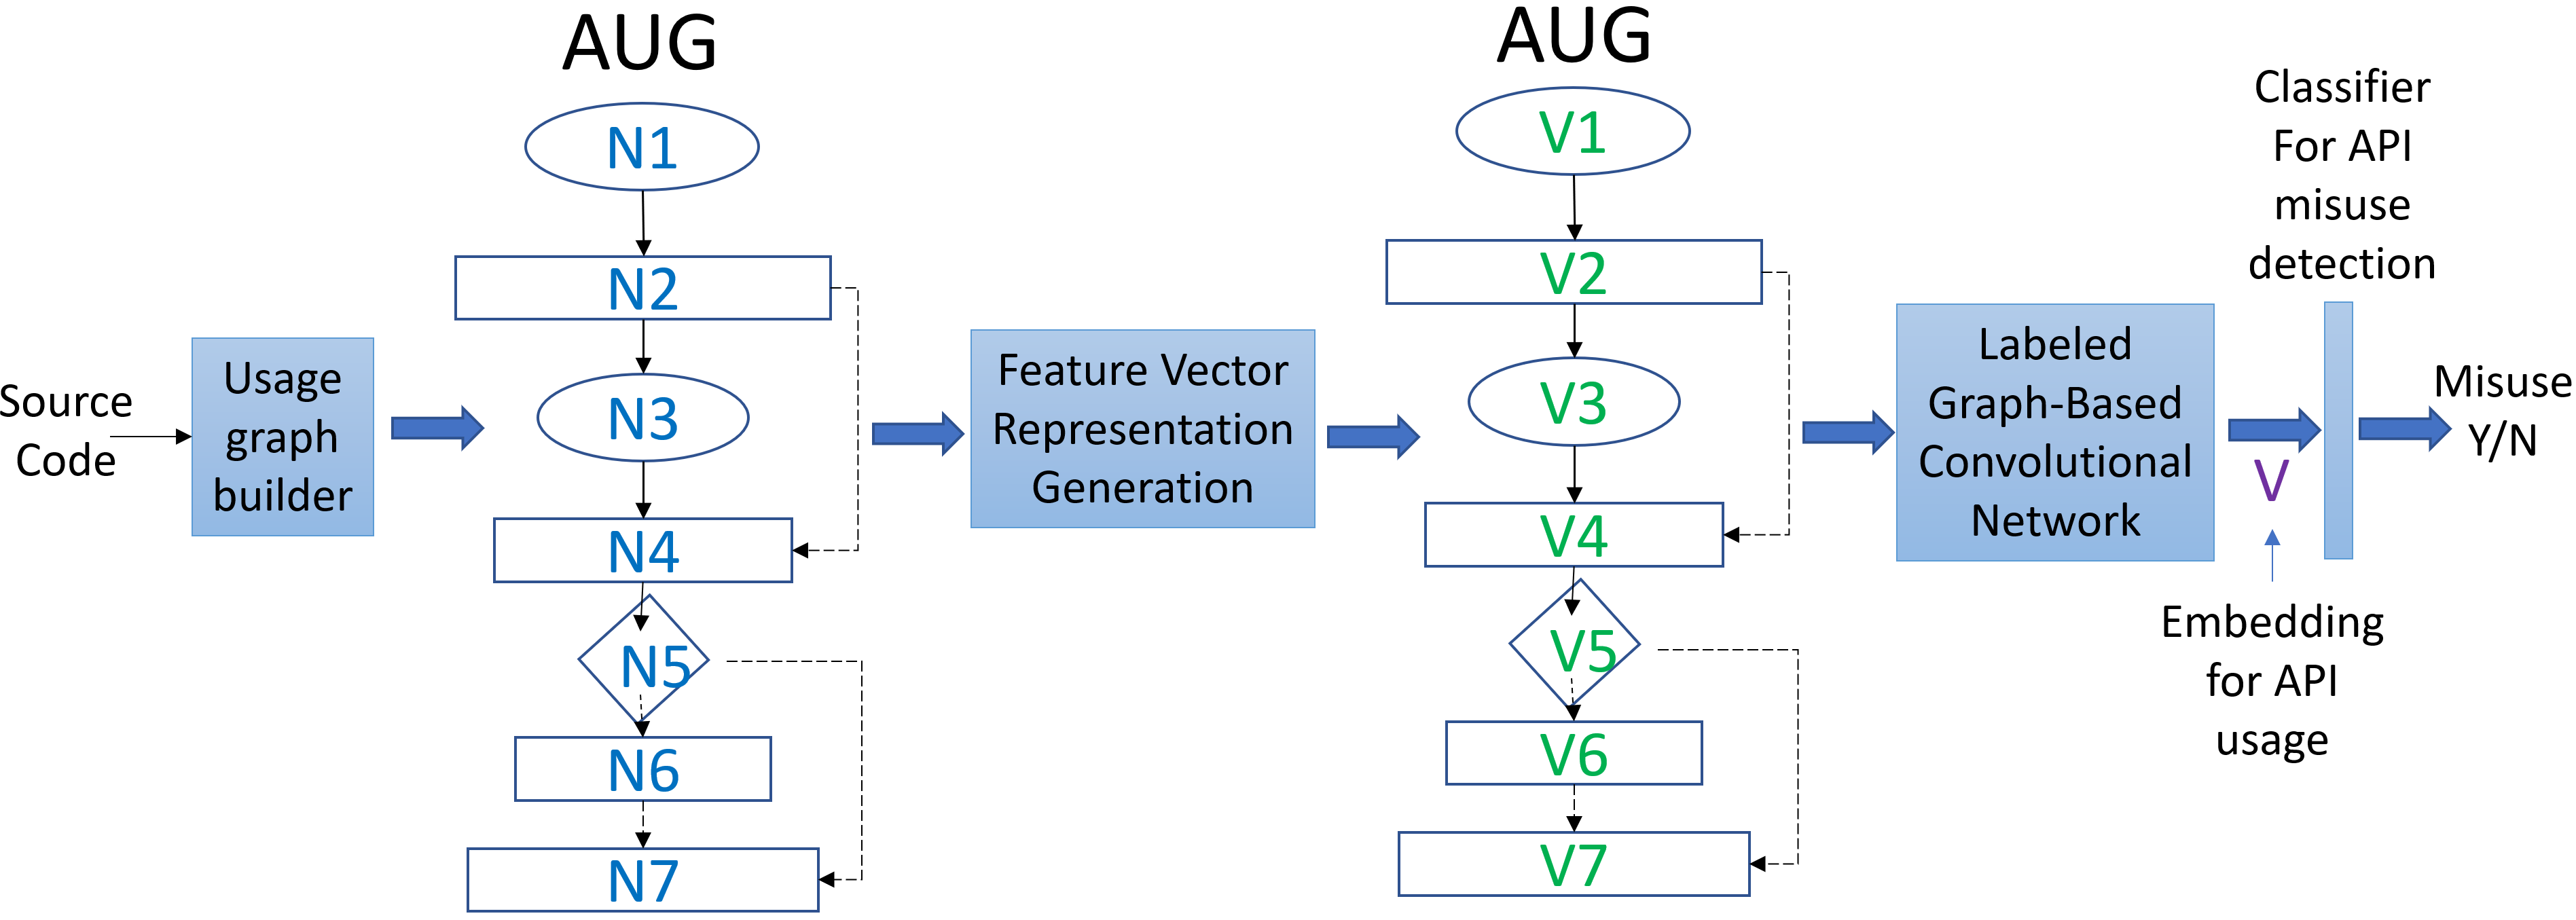
\includegraphics[width=5.6in]{overview.png}
\vspace{-5pt}
\caption{{\tool}: Architecture Overview}
\label{fig:overview}
\end{center}
\end{figure*}

In general, in addition to data augmentation component, {\tool} has
two main components (Fig.~\ref{fig:overview}). The first component is
to generate the usage graphs (AUGs) for all the methods. We use the
AUG building algorithm described in the original
paper~\cite{msr19}. The second component is to generate the feature
vector representations for all the nodes in the AUG. The output of
this step is the AUG in which the nodes $N_i$s are replaced by their
vector representations $V_i$s. This graph is then used as the input of
the third component, a Labeled Graph-based Convolutional Network
(Label-GCN)~\cite{label-gcn}, which is capable of learning the graph
structure among the nodes. From the representation vectors for all the
nodes in the AUG, the Label-GCN model will produce the outputs at the
output layer. The Label-GCN model connects all of its outputs to a
fully connected layer to transform the matrix into a vector $V$ for
the given API usage. This vector $V$ is the contextualized embedding
representing the given API usage. Our model then performs
classification by using a softmax function on $V$ to decide if it
contains an API misuse. In training, we use the labels of the API
misuses and benign usages.

Our model is also capable of identifying the API elements that were
misused. For that, in Fig.~\ref{fig:overview}, we do not connect all
the outputs of the Label-GCN to a fully connected layer. Instead, we
use the output nodes of the Label-GCN model to represent the decisions
of misuses or not for the corresponding API elements. In this case,
for training, we use as labels the misused API elements in each method
in training data. Then, for each output node of the Label-GCN model,
we use a softmax function to classify the node (i.e., the API element)
as misuse or not. For clarity, we do not show this case in
Fig.~\ref{fig:overview}.

